\chapter[Introduction]{Introduction}


\begin{flushleft}
\begin{minipage}[t]{0.80\textwidth}
\textit{It is true that there is no art without emotion\\
And there is no precision without craftsmanship\\
Just as there are no guitars without technology\\
Nylon technology for the high strings\\
Metal technology for the headstock\\
The press, the chisel, and the varnish\\
The carpenter's tools\\
The composer and his computer\\
The shepherd and his shaver\\
The alarm clock, announcing dawn\\
And in the telescope, the last star lingers\\
The machine is made by man\\
And it is what man makes of it}
\end{minipage}

\medskip
\hfill---Jorge Drexler, "Mi Guitarra y Vos"
\end{flushleft}

\bigskip

I vividly remember the first time I interacted with a language model. It was early 2019, and the model, GPT-2, was an early implementation of the novel transformer architecture leveraging the now-famous attention mechanism. It felt like a distinct experience. Back then, this model was open source, and to run it I had to download the model weights and scrape together a way to run it on a GPU, which I did with the help of a friend. It was not a particularly smooth experience, though it was exciting to be wrangling a neural network that somehow encoded the capability of producing language.

This model was rudimentary; when generating long sequences it often yielded nonsensical results and tended to go off in divergent directions. But it certainly had unprecedented language capabilities, sometimes generating text undistinguishable from that written by a person. This capacity, the ability to produce language, was previously thought exclusive to humans. Not anymore. Perhaps even more interestingly, interacting with these generative language systems often yielded genuinely interesting ideas \textit{in my own mind}.  The experience made me want to devote my work and research to the field of artificial intelligence and how humans can interact with it in creative and beneficial ways.

A few months later, in mid-2019, as I was applying to a master’s at the Australian National University’s 3A Institute to study the development of responsible AI-enabled systems, I decided to write my essay using GPT-2 as a "co-author", which proved both technically difficult and creatively rewarding. I wrote the first paragraph, which I fed to the model to generate the second paragraph, and so on. The topic was the potential implications of humans and AI interacting to co-create.

The whole process was disclosed and documented, and the code I used was provided with instructions on how to replicate exactly the text I generated. This was submitted alongside my essay, and a description of my iterative approach. Sometimes the paragraphs were not interesting, so I generated them again. At other times, they suggested ideas that opened up new possibilities, leading the essay in new directions. The most significant one was the suggestion, by the model, that \textit{language is the first technology}. Regardless of the anthropological validity of this claim, it made me reflect on the ironically profound implications of interacting with a technology that can produce language.

I eventually received an offer to the master’s and travelled from Mexico to Australia, arriving in early 2020, just a few weeks before the pandemic. After finishing my masters, I began this PhD research in late 2021 focused on enabling human-AI co-creativity. I finalised writing this thesis in 2025. In that relatively short period, progress in AI accelerated rapidly. Generative AI, which only a few years ago consisted of rudimentary models mostly used by curious neural network wranglers like myself, are now commonplace, used by hundreds of millions of people.

These generative capabilities of these models, across not only language, but also music, images, videos, music, code, and more, raise many pressing ethical, philosophical, and economic questions. They also open up the possibility of human-AI co-creativity.

The PhD research presented in this thesis is concerned with this possibility. In particular, it explores how to design generative AI systems that function effectively as co-creators, augmenting human creativity and preserving user agency, while allowing users to harness the creative potential of these technologies. It is also a practice-led exploration, in which, through my own creative work, I explore the potential and limitations of generative artificial intelligence as a co-creator. 

\section{Background}

In the field of natural language generation, neural networks have evolved from producing short, minimally coherent text sequences \cite{Bengio2003-xn, Sutskever2011-ne, Graves2013-yv} to large language models (LLMs) capable of achieving near, at or past human-level performance on complex tasks \cite{Vaswani2017-pb, Brown2020-js, Thoppilan2022-jf, OpenAI2023-lt, Anthropic2024-tc, DeepSeek-AI2025-ai, Gemini-Team2024-wk}. Today, LLMs can generate entire essays, pass advanced academic examinations at the PhD level, write software code at or above human proficiency, compose whole-length novels, engage in multi-step reasoning, and understand and reason across images, audio, and video \cite{Gemini-Team2023-ux, OpenAI2024-em}. 

In terms of creative capabilities, a recent study by Hubert et al. reported that an LLM outperformed humans in standardised tests of creativity and divergent thinking \cite{Hubert2024-kv} while another study by Guzik et al \cite{Guzik2023-cl} reported that an LLM scored in the top 1\% for originality and fluency in the Torrance Test, a standardised assessment used to measure human creativity. 

The field of image generation has similarly made significant strides. Neural networks went from producing rudimentary images \cite{Goodfellow2014-jz, Mordvintsev2015-oz} to modern diffusion models capable of generating photorealistic images often indistinguishable from genuine photographs, and to produce images in a variety of artistic styles \cite{Ramesh2021-xb, Rombach2021-wf, Ho2020-zj, OpenAI2021-te, Nichol2021-ne, Zhang2023-by}. In a recent survey with more than 11,000 participants, humans were not reliably able to distinguish AI generated art from paintings made by humans. Moreover, participants tended to rate AI-images slightly higher in preference \cite{Alexander2024-pz}. Similar progress is evident in music generation, where AI has progressed from creating simple melodies \cite{Huang2018-pc, Dhariwal2020-au, Roberts2019-ym} to full-scale songs \cite{Copet2023-mh, Suno2024-wa, Udio2024-rc}. Currently, emerging video-generation models such as Gen3-Alpha, Sora, MovieGen suggest the extension of this trend to the moving image domain \cite{Runway2024-zs, Polyak2024-lh, OpenAI2024-ua}.

\begin{figure}
    \centering
    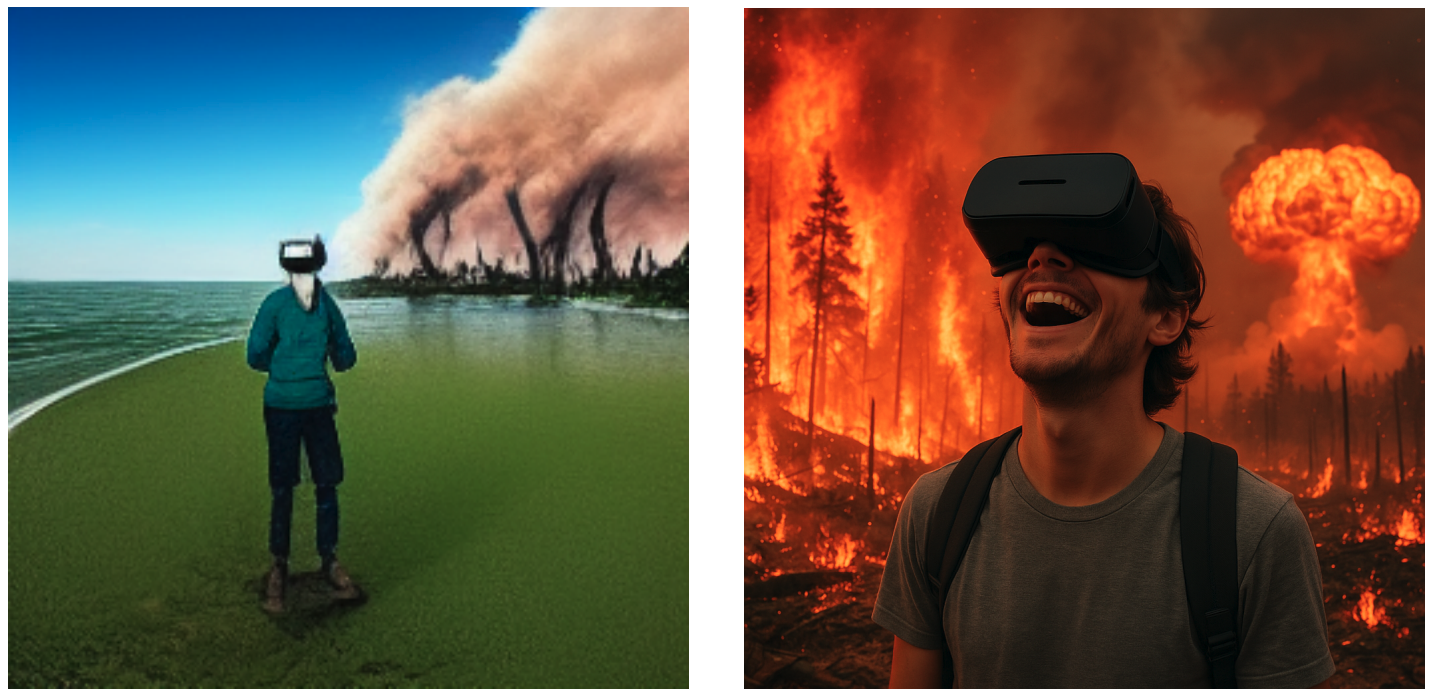
\includegraphics[width=1\linewidth]{comparisonimages.png}
    \caption{An illustration of the rapid developments in generative AI that took place in the time period spanning this thesis. \textbf{Left:} generated by the author in June 2022 using the prompt: "A person with a VR headset in the middle of an ecological catastrophe". \textbf{Right:} generated by the author exactly three years later, in June 2025.}
    \label{fig:enter-label}
\end{figure}

These technologies have not stayed in the lab; increasingly, they are becoming widely adopted and a part of everyday life for millions of people. A report by the UBS firm estimated ChatGPT reached 100 million users two-months after launch, making it the fastest application to reach this milestone \cite{Hu2023-ie}. Today, educators employ tools like ChatGPT and other chatbots to develop lesson plans, students leverage it for essay writing, doctors are using it to generate discharge summaries \cite{Patel2023-fg}, researchers use it to locate scholarly information and draft manuscripts, programmers are using it to write code, and laypeople are using it to ask questions, brainstorm ideas, write emails, among many other uses. 

Image-generation tools such as Leonardo, MidJourney, DALL-E, and Stable Diffusion have garnered significant user bases. According to a recent survey by Adobe (2024), approximately 40\% of designers have incorporated some form of generative AI into their design processes \cite{Offerman2024-lf}. People use these tools to create art, ideate designs, reimagine interior designs, create materials for presentations and more. 

As capabilities and adoption rise, AI is poised to become one of the most transformative technologies in modern history. Among the many questions raised by these developments, including ethical, political, economic, and environmental, one of the central ones is: How will generative artificial intelligence influence and intersect with human creativity, and how can we leverage it effectively while maintaining creative agency?

\subsection{Creativity, Technology and Artificial Intelligence}

Historically, technology and creativity have co-evolved in complex and intertwined ways. Almost all human creative activities rely on tools, and new technologies invariably open up novel creative possibilities and practices. However, new technologies can also lead to the automation of part of the creative process and in some cases, the replacement of human creators.

The invention of the camera provides an illustrative example. As a technology, the camera was initially partly met with resistance. The French poet Baudelaire famously argued that the purely material applications of photography would be detrimental for art \cite{Baudelaire1955-ae}, and art critics and theorists criticised the effect of the mechanisation of visual production such as in Walter Benjamin's famous essay The Work of Art in the Age of Mechanical Reproduction \cite{Benjamin1935-wd} . Photography did indeed supplant some traditional painting practices. Hand-painted magazine illustrations and commercial art, once a vital source of income for artists like Magritte in the early stages of their careers, are now predominantly produced through photography and digital methods. 

However, the camera also expanded creative possibilities by enabling the rise of photography and later film as rich new artistic practices in their own right. In a more nuanced way, photography influenced painting, and painting influenced photography, pushing each other in new directions . In his book "Art and Photography", Aaron Sharf discussed the mutual artistic influence of photography and painting, and described how the camera led to painters to reconsider and develop their techniques by providing them with new perspectives and reference material \cite{Scharf1968-na}. The rise of Impressionism, can be, at least to some degree, understood as the practice of painting occupying a less literal niche to visually capture reality. For Vincent Van Gogh, the advantage of Impressionism was that it provided "a deeper resemblance than the photograph" \cite[p. 116]{Marmor1997-ka} and for photographer Henry Peach Robinson, Impressionism did good to photography by showing "we should represent what we see, and not what the lens sees" \cite[p. 87]{Robinson1896-mo}. 

Artificial intelligence may interact with human creative practices in similar ways. It may automate some creative practices completely, support existing ones, and become a tool for new creative practices altogether. In this thesis, I am concerned with a distinct possibility that may integrate aspects of all them but also open new avenues for the co-evolution of creativity and technology: that of \textit{\textbf{co-creativity}}. In co-creative interactions, the technology itself exhibits creative capacities and is able to collaborate synergistically with human creators.

\subsection{Human-AI Co-Creativity}

Candy \cite{Candy2002-ra} described \textit{co-creativity} between people as a closely woven interaction that produces an output as a result of a symbiotic combination of actions. Creative participants align goals and intentions, collaboratively moving towards an outcome. In recent years, the field studying the potential for co-creativity between humans and machines has grown. 

Davis \cite{Davis2013-jy} first introduced the concept of human-computer co-creativity, describing an interaction where the computer is not just a rigid executor but adapts dynamically, drawing on computational creativity algorithms to respond to the user. Since then, across a growing literature, authors argue for the potential of human-AI co-creativity as a scenario that can augment, enhance and support human creativity, mitigating many of the risks posed by this technology while unlocking the beneficial opportunities it provides.  \cite{Yannakakis2014-zs,Kantosalo2020-zf,Rezwana2022-gg,Moruzzi2024-cq,Haase2024-yp,Lin2023-zq,Karimi2018-wi,Vinchon2023-gh}. Various definitions have been proposed for human-AI co-creativity. Drawing from them, I provide the following definition in my own terms to be be used throughout this thesis: 

\begin{quote}
\emph{A type of human-AI interaction involving creative contributions from both human and AI and where the outputs cannot be uniquely or primarily attributed to the creative behaviour of one of them.}
\end{quote}


This choice in definition and term usage of "creative contributions" and "creative behaviour" is motivated by three main characterisations in the literature of human and machine creativity. 

First, by the widely accepted characterisation of something as creative if it is both \textbf{novel (or surprising)} and \textbf{valuable (or appropriate)} \cite{Amabile1983-lj, Sternberg1998-oz, Runco2012-mk, Boden2003-hk}. As such, I refer to a \textit{creative contribution} as one that satisfies this double constraint, and \textit{creative behaviour} as a process that can produce it. 

Acknowledging that novelty and value depend on frames of reference, my own definition of co-creativity considers the working definition of computational creativity offered by Colton and Wiggins' \cite{Colton2021-bt} as observer dependent.  They define computational creativity as:

\begin{quote}
The philosophy, science and engineering of computational systems which, by taking on particular responsibilities, exhibit behaviours that unbiased observers would deem to be creative.
\end{quote}
 
Thirdly, I draw from Rhodes' \cite{Rhodes1961-od} 4P's of creativity, which later Jordanous re-conceptualised for computational creativity \cite{Jordanous2016-xb} and which I here defined in my own terms: 

\begin{itemize}
    \item Person/Producer: The features of the system that make it capable of a particular creative behaviour and contributions.
    \item Process: The methods, strategies and algorithms used to drive creative behaviour and contributions.
    \item Press: The environment environment in which a generative system acts, including its interaction with the user and influences its creative behaviour and contributions.
    \item Product: The outputs produced from the interactions between the above resulting in creative behaviour and contributions.
\end{itemize}

Lastly, my understanding of creativity is heavily informed by Bown's notion of distributed creativity, as a process not exclusive to humans, which can be observed in natural and artificial systems (individual and collective), and which considers creativity as emerging from interactions within networks of distributed agency rather than emanating from individuals \cite{Bown2012-gg, Bown2021-os}. 

As such, human-AI co-creativity is a type of emergent and relational creativity, which, as other authors have suggested, can be attributed not to any of the agents but rather to the ensemble of interacting agents as a whole \cite{Davis2013-jy, Rezwana2023-rt}

Through his concept of Material Agency, Lambros Malafouris argues that a craftsman is influenced by his tools and materials as much as he is influenced by them \cite{Malafouris2013-by}. This idea similarly underpins the concepts of Extended Cognition and Extended Mind Theories, both highly influential in creativity studies and which posits that tools and environments are extensions of a person's mind \cite{Clark1998-yi}. A natural question arises then: how is the emergent co-creativity of a human-AI interaction different from that of a person creating with their tools in a mutually influencing loop? Crucially, the difference is that in this case, the tool is capable of creative behaviour itself. According to the definitions of creative behaviour provided above, it becomes increasingly evident that this is the case. 

\subsubsection{Machine Creativity?}

Achieving creative behaviour was an explicit goal of the founding project that first coined the term and defined the field of artificial intelligence: the Dartmouth Summer Research Project on Artificial Intelligence \cite{McCarthy1955-ls}. Since then,  many researchers have sought to describe how computers could act creatively and how this creativity can be measured \cite{Boden2003-hk, Boden1998-yn, Colton2012-jc, Bown2012-gg, Moruzzi2020-mw, Wiggins2006-zd, Jordanous2012-kw}. However, machine creativity has long been considered one of the final frontiers in artificial intelligence \cite{Colton2021-bt},

In 2016, AlphaGo decisively beat the top human player in the world of Go. Throughout this match, AlphaGo was observed to play highly unexpected but effective moves, thus satisfying the constraint for novelty and value. One example is the now famous \textbf{move 37}, an extremely unexpected move made by AlphaGo that ended up turning the game in its favour. One commentator narrating the game described it as "a very strange move," while another claimed he thought it was a mistake. After the move materialised its game-defining value, another commentator claimed: "It’s not a human move. I’ve never seen a human play this move. So beautiful."

While AlphaGo first learned from human match data, its success resided in a step of reinforcement learning, where it played against itself. This helped it identify moves that could be successful even if never played by a human. It was this how it arrived to the game defining move 37, which was calculated to have 1 in 10,000 chance of being played by a human in that situation. A common counterargument to the possibility of AI creativity is that these algorithms only learn from human data and thus can only produce outputs that plausible replicate them. However, the AlphaGo example showcases the possibility of behaviour in machines that produce surprising, novel an valuable outputs \textit{and} that are highly different from that which a human would do.

Today, advances in generative AI reinforce the possibility of creative behaviour in other fields. As mentioned above, LLMs have now outperformed humans in some standardised tests of creativity and divergent thinking, such as the Alternative Uses Test and Torrance Test, in some case scoring in the top 1\% for originality and fluency \cite{Hubert2024-kv, Guzik2023-cl, Koivisto2023-lw}. Turing-style tests have shown humans have a hard time distinguishing art generated with AI and art generated by humans \cite{Alexander2024-pz}. 

While this may paint primarily a future of displacement of human creativity by automated means, the emergence of machine creative behaviour has also begun to opens the possibility for machine creativity that helps expand human creativity and synergise with it. 

\subsection{The case for human-AI co-creativity}

While AlphaGo decisively defeated the top human player in the world exhibiting moves that could be deemed creative, Metz \cite{Metz2016-dm} reported how AlphaGo has itself helped Go players see the game differently and improve as a result. In the field of creative writing, a study by Hitsuwari \cite{Hitsuwari2023-tw} showed that Haikus written in close cycles of iteration between humans and AI were rated higher than either writing Haikus alone. Increasingly, a growing creative artistic practice, including my own, has seen artists engaging AI technologies in co-creative ways, and using them to enable new previously unfeasible possibilities. 

Recent evidence suggests that beneficial outcomes are achieved when humans and AI are engaged in close cycles of collaboration and interaction, as opposed to each solving problems that require creativity on their own. A systematic study published in Nature by \cite{Vaccaro2024-ne} found evidence for what they term "human-AI synergy", measured as greater performance of Human and AI compared to Human or AI acting alone in the field of content production. A study done in collaboration between Harvard Business School and international consulting firm Boston Consulting Group looked at the effect of 758 consultants leveraging LLMs. They found that close synergies between humans and LLMs led to the highest outcomes compared to humans alone and to humans simply outsourcing tasks to the LLM with minimal involvement \cite{DellAcqua2023-og}. In a similar finding, McGuire \cite{McGuire2024-im} showed that when humans assume more passive roles of outsourcing creative production in  the case of writing, creative self efficacy and feelings of agency diminish, but when the interface facilitates them engaging as active co-creators, their creative self efficacy improves, as well as the measured outcomes. 

However, enabling such co-creative interactions is not trivial, and many challenges lie ahead. 

\subsection{Problem Statement: The Challenges of Human-AI Co-creativity}

With this, we arrive at the problem definition, which presents the central challenge in designing effective co-creative AI and which represent the central challenge addressed in this thesis. Broadly, it can be divided in two: challenges concerning the human user, and those concerning the co-creative system itself itself.

\subsubsection{Human Side}

Humans often over-rely on automated systems, leading to \textbf{minimal involvement} and, ultimately, a loss of skill and agency. In a study by Gerlich \cite{Gerlich2025-as} involving 666 participants, increased use of language models correlated with decreased critical thinking skills, apparently due to cognitive offloading. Similarly, a study by Carnegie Mellon and Microsoft Research found \cite{Lee2025-dw} that higher confidence in generative AI correlated with decreased measures of critical thinking. Conversely, another large-scale study by Essel et al. \cite{Essel2024-qc} reported the opposite effect in a controlled setting: students who engaged with a chat-based language model, and who received a pre-written set of prompts designed to stimulate critical reflection with the model, showed greater measures of critical and creative thinking.

These conflicting findings suggest that outcomes depend heavily on \emph{how} users interact with AI, which can be shaped by interface and interaction design but also personal motivations and context \cite{Lehmann2022-kr, Kantosalo2020-nh,Liapis2016-bv,Lin2023-jd,Karimi2020-cf,Moruzzi2024-cq, Rezwana2022-gg,Abbas2024-sf}. For example, while trust in the AI system can lead to greater overreliance, research shows that trust is important for effective co-creation \cite{McCormack2019-yh, Louie2020-aq, Kruger2017-xa, McCormack2020-ix, Hutchings2020-bv, Wang2020-cw, Rezwana2022-ui}. 

These nuances and potential contradictions highlight how it remains unclear how best to design systems and interfaces to foster active user engagement and co-creativity. 

\subsubsection{AI Side}
Generative AI systems themselves also pose several challenges for co-creativity. Chief among these are difficulties in controlling and steering outputs—leading some practitioners to describe them as “slot machines” \cite{Nebelong2023-rb}—and a lack of support for the iterative, evolving nature of the creative process \cite{Park2024-gw}. Moreover, they are often viewed as “black boxes” with low interpretability \cite{Llano2022-ti, El-Assady2022-qc}, can produce overly generic outputs that some practitioners feel lack a “human touch” \cite{Park2024-gw}, and may override or overwrite user-created content in undesirable ways \cite{Buschek2021-ks}.

In addition, while forming mutual understanding is crucial in collaboration and creativity, generative systems often struggle to grasp nuanced human goals \cite{Bown2024-yx}. Furthermore, in human–human co-creative scenarios, collaborators can challenge one another and offer perspective shifts that drive the creative process forward. By contrast, generative systems are typically trained to strictly follow user instructions \cite{OpenAI2022-pj} or user prompts \cite{Ramesh2022-kc}, limiting their potential to help users explore genuinely novel or unexpected directions.

These challenges are multi-faceted and can be approached from various angles. In this thesis, they are examined through the lens of interaction design and practice-based research. 

\section{Approach}

\subsection{Hypothesis}

To address the previously highlighted challenges, I began with the hypothesis that \emph{dialogic interaction} can mitigate many of these limitations. This hypothesis is informed by the observation that traditional interactions with computers, including generative systems, typically follow a linear pattern in which a command is given and an output is returned (see Figure \ref{fig:unidirectional}). 

\begin{figure}[hbt!]
    \centering
    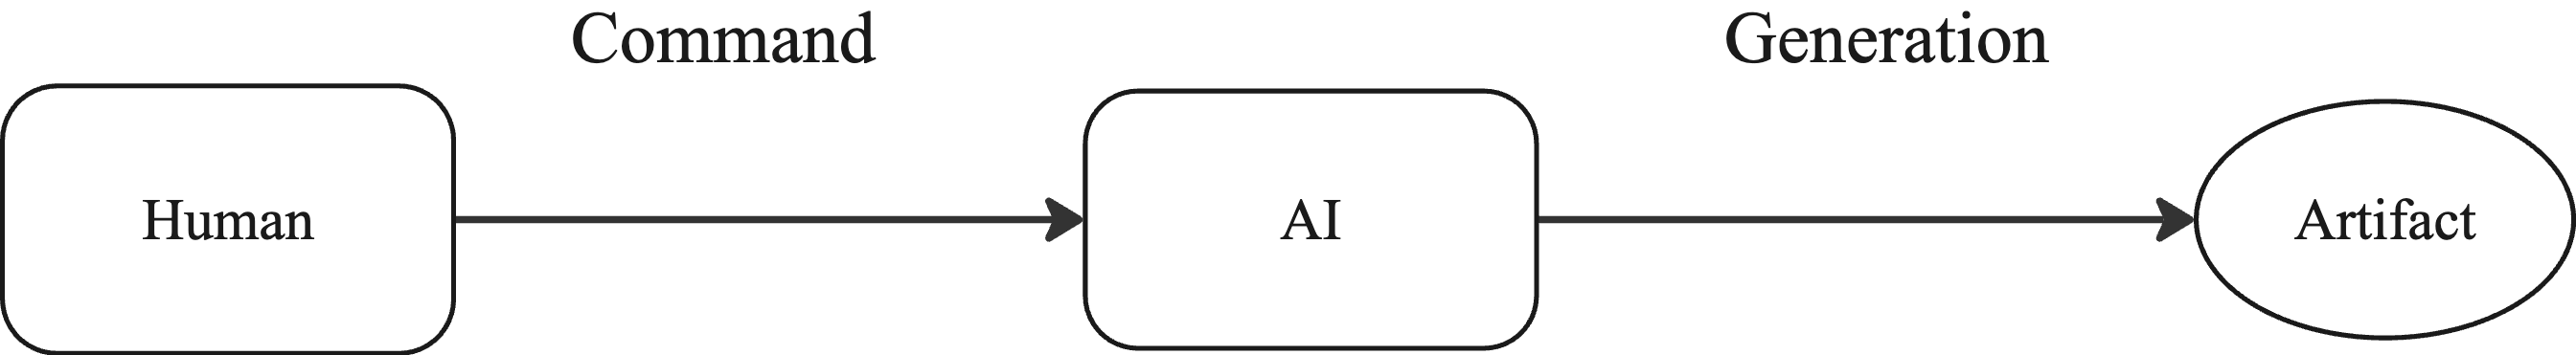
\includegraphics[width=0.75\linewidth]{unidirectional.png}
    \caption{Example of an unidirectional interaction with a generative AI system}
    \label{fig:unidirectional}
\end{figure}

However, as computers increasingly exhibit creative potential, the conventional command--execute paradigm becomes insufficient for fostering collaborative relationships. Instead, effective \emph{co-creative} engagement calls for \emph{dynamic back-and-forth conversations}, wherein both human and AI agents participate in iterative cycles of mutual understanding and influence. This is what I refer to by dialogic interaction. Importantly, in a dialogic process, participants can communicate \emph{both through} the creation itself and \emph{about} the creation (see Figure \ref{fig:dialogicthroughandabout}), thereby enabling deeper collaboration. As such, conversation may be a part of it, but not the exclusive component. 

\begin{figure}
    \centering
    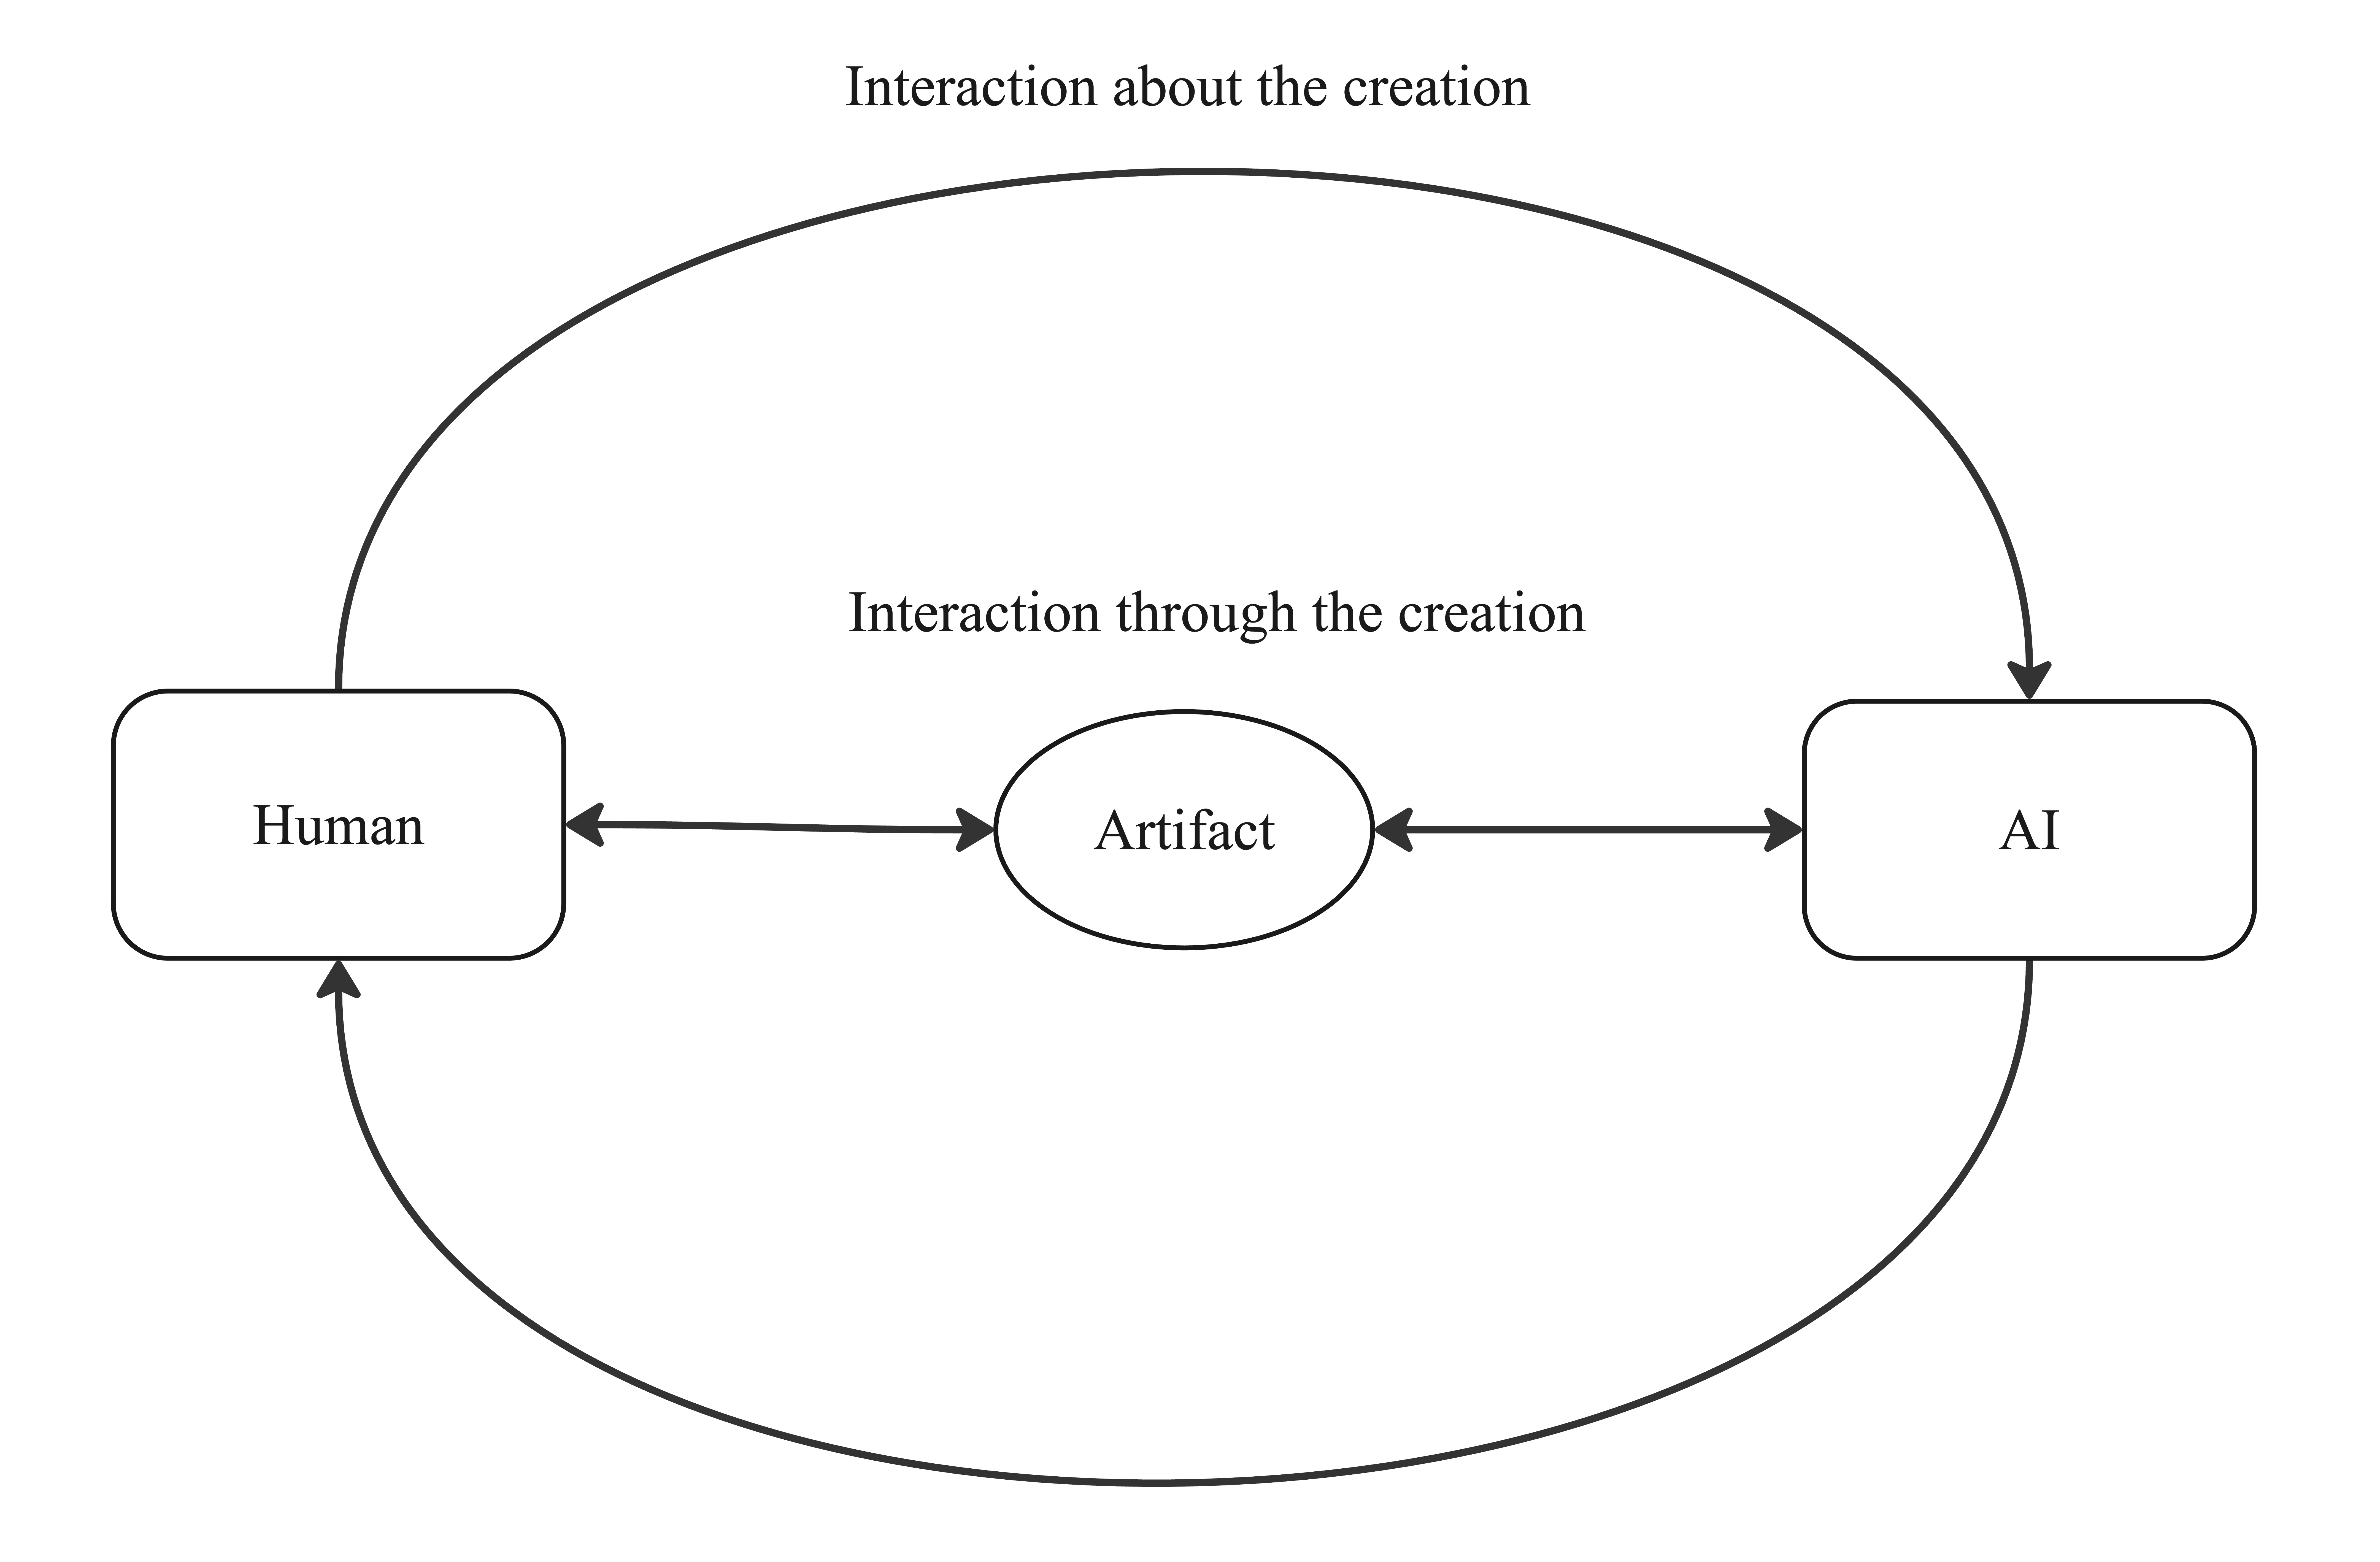
\includegraphics[width=0.75\linewidth]{dialogicthroughandabout.jpg}
    \caption{Diagram showing a dialogic interaction between a human and generative AI system interacting through and about the creation}
    \label{fig:dialogicthroughandabout}
\end{figure}

Dialogue has long been discussed in fields such as Human--Computer Interaction (HCI) and creative practice as a means to model interactions with computers and creative tools. Despite this, it remains underformalised as an interaction design concept in HCI. My research, conducted as part of an Australian Research Council (ARC)-funded project exploring Dialogic Creative AI, builds on initial work by Bown et al \cite{Bown2020-oc} to address this gap.

In light of the emergence of chat-based interfaces as the predominant mode of interaction with language models, it might seem self-evident that dialogic interaction can enhance co-creativity. However, my characterization of dialogue extends beyond bidirectional text exchanges. By drawing on philosophical, educational, and interdisciplinary dialogue literature, I develop a more comprehensive construct of \emph{dialogic interaction} comprising six key elements:

\begin{itemize}
    \item Bidirectional communication
    \item Shared collaborative space
    \item Iteration
    \item Mutual Influence
    \item Mutual Understanding
    \item Context-awareness
\end{itemize}

These elements are discussed in detail in Chapter~3. Notably, while bidirectional textual exchanges (as exemplified by popular chat interfaces) constitute one component, my proposal predates the widespread adoption of chat-based interactions, including the late 2022 launch of ChatGPT. The public success of such interfaces underscores the value of \emph{one} aspect of dialogic interaction (two-way communication) yet other elements remain to be explored. Throughout this thesis, I examine how these additional elements can further support effective human--AI co-creativity.

Against this backdrop, I formulated one overarching research question and three sub-questions to guide this inquiry:

\begin{quote}
\textbf{Core Research Question:}
\emph{How can we design generative AI systems that act as effective co-creators, maintaining human agency while effectively leveraging the creative potential of this technology?}
\end{quote}

\begin{quote}
\textbf{Sub-Questions:}
\begin{enumerate}
    \item \textbf{R1:} \emph{How does interaction design influence the role that humans and AI play in creative production?}
    \item \textbf{R2:} \emph{What is the potential of modelling dialogue in interaction design to enable effective human–AI co-creativity?}
    \item \textbf{R3:} \emph{Which interaction design principles can guide the development of effective co-creative systems?}
\end{enumerate}
\end{quote}

\subsubsection{Methodology}
To address my research questions, I adopt a mixed-methodology approach integrating qualitative and quantitative research methods across two strands: interaction design research and creative-led practice.

I focus specifically on human–AI co-creativity within three creative domains: writing, image generation, and interactive new media music installations. On one hand, I develop prototypes that are tested with users to evaluate the potential of dialogic interaction in enabling human–AI co-creativity. On the other hand, I engage in a creative practice-led approach by developing interactive artworks and collaborating with professional creatives in the completion of projects leveraging generative AI, which I then analyse as case studies. Through these analyses, I discuss both the potential and the limitations of these systems to be co-creative in real-world scenarios, with particular emphasis on dialogic interaction.

A diagram illustrating the approach and methodology is shown in Figure \ref{fig:approach_figure}.


\begin{figure}
    \centering
    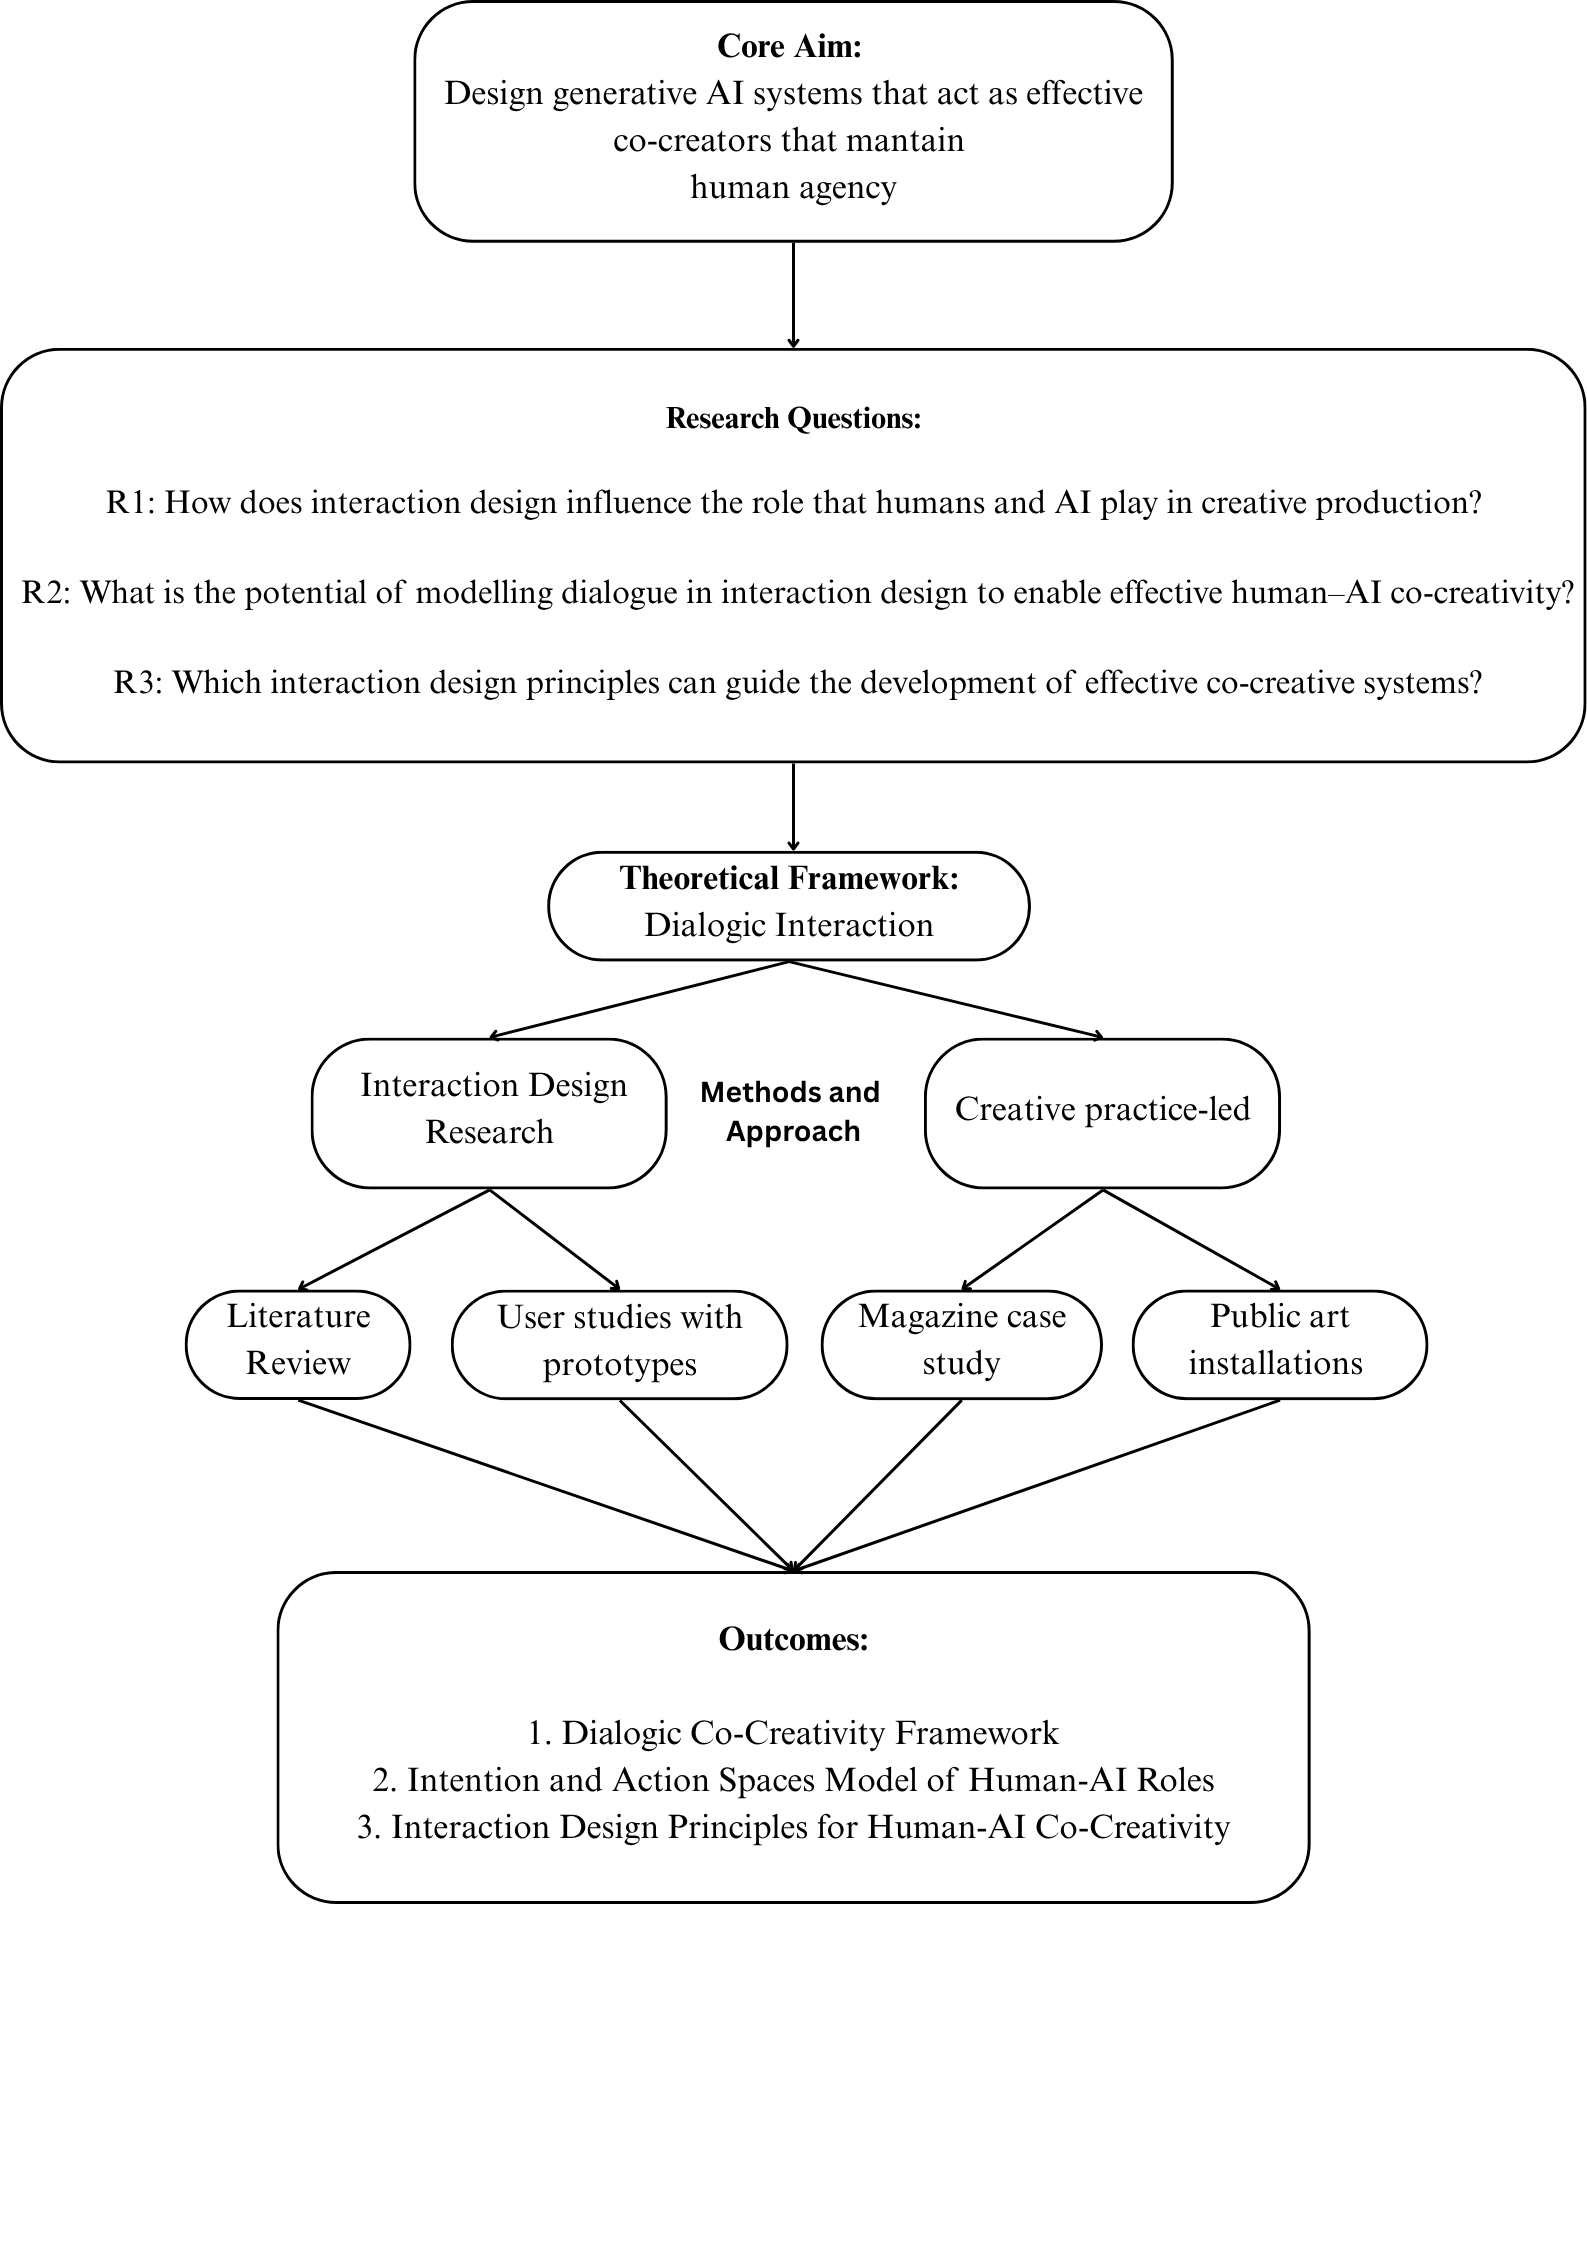
\includegraphics[width=1\linewidth]{DiagramStructure.png}
    \caption{Diagram illustrating the research approach, from the core aim to outputs}
    \label{fig:approach_figure}
\end{figure}

\section{Thesis Structure}

This thesis is structured chronologically but not strictly so, as I prioritised grouping studies by creative practice: writing, image generation, and public art installations. As such, the three primary study chapters (Chapters 4, 5, and 6) are organised accordingly. The preceding chapters establish the theoretical foundations that underpin the thesis (Chapters 2 and 3), while the final chapter (Chapter 7) integrates the findings and conclusions.

\subsection{Chapter 2: Literature Review}

Chapter 2 reviews the literature relevant to the three research questions, covering a multidisciplinary literature across human creativity and computational creativity, human-computer interaction and emerging literature on human-AI co-creativity. The review is structured in two main parts: the first establishes foundational concepts by defining human-AI co-creativity and creativity more broadly, before identifying the current gap in design principles for co-creative systems. The second part then addresses the three research questions in reverse order, beginning with design principles, then exploring the potential for dialogic interaction, and concluding with an analysis of roles in human-AI co-creative processes. A key finding is that while numerous interaction design principles exist in HCI, no such principles exist yet specifically for human-AI co-creativity, representing a significant gap this thesis aims to address.

\subsection{Chapter 3: Dialogic Human-AI Co-Creativity}

Chapter 3 addresses research subquestion 2 regarding the potential of modelling dialogue in interaction design to enable effective human-AI co-creativity. It is presented in two parts. The first consists of a paper from the 2022 CHI GenAI workshop, which served as an initial exploration of how dialogue could enhance collaboration with generative AI. At the time, I explored repurposing text-completion functions to engage with models in a dialogic way, arguing that effective co-creativity requires mutual understanding that dialogue can facilitate. A key output was a typology of actions that both humans and AI could engage in during creative dialogue.

The second part presents a more comprehensive framework for dialogue as an interaction design concept, proposing that Dialogic Co-Creativity involves interaction \textit{through} and \textit{about} the creation and comprises six key components: bidirectional communication, shared space, iteration, mutual influence, mutual understanding, and context-awareness. These components form an analytical lens for the subsequent empirical chapters, which explore their implementation and contribution to effective human-AI co-creativity.

\subsection{Chapter 4: Beyond Chat: Collaborative Editors Enhance Human Involvement and Agency When Co-Writing with Large Language Models}

Chapter 4 focuses on the writing domain and addresses the core research question by examining interfaces that preserve human creative agency. Following the widespread adoption of chat-based conversational interfaces as the dominant mode of interaction with LLMs, I hypothesised that an interface providing a collaborative space could better support interaction both \textit{through} and \textit{about} the creative product. The chapter presents two user studies evaluating prototypes (Vorges and Common AI) that combined chat interfaces with collaborative text editors, allowing both users and AI to discuss and directly edit text.

Results demonstrated that chat-only interfaces restricted user agency and involvement at the writing level, while the hybrid interface resulted in users reporting higher levels of agency and active involvement in the co-creative writing process. The findings reveal how interaction design influences the roles assumed by humans and AI, with chat-only interfaces positioning users primarily in directive roles while the hybrid interface encouraged more balanced participation in the actual writing process.

\subsection{Chapter 5: Integrating Generative AI into Creative Workflows: Dealing with Consistency, Scene Control, and Refinement in a Professional Image Generation Case Study}

Chapter 5 shifts focus to image-based generative AI through a practical case study involving real-world creative production. I collaborated with the Australian Financial Review to produce visuals for their annual Power Issue, aiming to create "impossible photography" of Australia's most powerful people that would tell stories about their personality and work in ways not possible with traditional photography. This exploration contributes to understanding effective human-AI co-creativity by identifying how generative tools can enable new creative possibilities and use cases.

The case study primarily informs the interaction design principles by highlighting crucial challenges in current tools. A significant limitation identified was the difficulty in enabling precise control over style and structure, particularly when relying solely on prompting interfaces. A second notable challenge was iteratively exploration and refinement, a crucial dynamic in creative processes that remains a critical challenge for successful human-AI co-creativity. The chapter also illuminates important ethical considerations around deepfakes and potential job displacement in creative industries.

\subsection{Chapter 6: New Roles for Generative AI Co-Creators: Two Case Studies in New Media Public Art Installations}

Chapter 6 describes the creation of two generative public art installations that leverage generative language models for real-time audiovisual performance. The first, commissioned for the ANU School of Cybernetics, generated soundscapes in response to environmental data including weather in Canberra, social media activity, economic indicators, and atmospheric CO2 levels. The second, commissioned for the Sydney Opera House, produced a continually evolving, month-long soundscape driven by data on the building's energy usage, performances, and water consumption.

These installations explore how generative artificial intelligence opens up new creative possibilities in new media practice by enabling AI to assume novel co-creative roles that humans currently do not assume. However, they also highlight ongoing challenges, as these systems remain difficult to steer towards human creative intent while maintaining responsiveness to their environmental context. The installations demonstrate the potential for context-aware co-creative systems while revealing the complexities of implementing such contextual responsiveness in practice.

\subsection{Chapter 7: Conclusion}

Chapter 7 presents the core argument of the thesis: that prevailing modes of interaction with generative AI often diminish user creative agency through what I term "severed creative agency"—a fundamental disconnect between a user's creative intentions and the actions performed by the AI. The chapter addresses the research sub-questions, beginning with an analysis of how interaction design shapes roles and agency, showing that humans increasingly operate in the \textit{intentional space} while AI assumes roles in the \textit{action space}.

The chapter then discusses how dialogic interaction can addresses this by facilitating more fluid movement between intentional and action spaces through context-aware, iterative interactions that promote mutual adaptation and understanding. As the main contribution, the chapter synthesises findings into a set of 11 actionable design principles for creating more effective co-creative AI systems, organised under four key dimensions: Iteration, Communication, Collaboration, and Integration. These principles provide concrete guidance for developing co-creative systems that maintain human agency while effectively leveraging the creative potential of generative AI.

%%%Chapter overview